
\documentclass[11pt,a4paper]{article}
\usepackage[left=2cm,right=2cm,top=2cm,bottom=2cm]{geometry}
\usepackage[utf8]{inputenc}
\usepackage[T1]{fontenc}
\usepackage[english]{babel}
\usepackage{setspace}
\usepackage{parskip}
\usepackage{enumitem}
\usepackage{hyperref}
\usepackage{mathptmx} 
\usepackage{csquotes}
%\usepackage[backend=biber,style=apa]{biblatex}
\usepackage[backend=biber,style=numeric]{biblatex}
\renewcommand*{\bibfont}{\small}  % Schriftgröße der Referenzen
\usepackage{soul} % us hl to highlight
\usepackage{xcolor} % Optional, falls du die Farbe ändern willst
\usepackage[most]{tcolorbox}  % in der Präambel
\usepackage{titlesec}
\usepackage{changepage}
\usepackage{comment}
\usepackage{tabularx}
\usepackage[table]{xcolor} % Optional: für dezente Hintergrundfarben
\usepackage{booktabs}      % Für schönere Tabellenlinien
\usepackage{longtable}
\usepackage{array}
\usepackage[table]{xcolor}
\usepackage{graphicx}   % wichtig fürs Einfügen von Bildern
\usepackage{caption}    % erlaubt auch unnummerierte Captions (optional)
\usepackage{wrapfig}   % Text um Bilder herum
\captionsetup[figure]{name=Fig.}
\captionsetup[figure]{aboveskip=1pt, belowskip=-2ex}
\captionsetup[figure]{font={scriptsize,it}}

% Vor der Tabelle:
\renewcommand{\arraystretch}{1.2}
\rowcolors{2}{gray!10}{white}

\titlespacing*{\section}{0pt}{0.8ex plus 0.5ex minus .2ex}{0.3ex}
\titlespacing*{\subsection}{0pt}{0.8ex plus 0.5ex minus .2ex}{0.3ex}
\titlespacing*{\subsubsection}{0pt}{0.8ex plus 0.5ex minus .2ex}{0.3ex}
\titleformat{\paragraph}[block]{\normalfont\normalsize\bfseries}{\theparagraph}{1em}{}
\titlespacing*{\paragraph}{0pt}{0.5ex plus 0.2ex minus 0.1ex}{1ex}

\sethlcolor{yellow} % Setzt die Highlight-Farbe
\setlist[itemize]{leftmargin=*, topsep=-3pt, itemsep=0pt}
\setstretch{1}

\addbibresource{/Users/sweis/Data/Arbeit/Bibliothek/NewMasterBib_LaTex.bib}

\begin{document}

\hl{Name, institution, and contact details of the applicant (one person only) and a list of the scientists or institutions involved in the research project (max. 2 A4 pages)
CVs and lists of publications need not be submitted.}

PD Dr. rer. medic. Susanne Weis, Heinrich Heine University Düsseldorf; \\
Gruppenleiterin „Variabilität des Gehirns“, Gehirn und Verhalten (INM-7), Institut für Neurowissenschaften und Medizin,  
Forschungszentrum Jülich; \\
E-Mail: S.Weis@fz-juelich.de

Simon

INM-7: The proposed work is embedded in a multidisciplinary working team combining knowledge in the field of neuropsychology, structural and functional MRI analysis, computational neuroscience and machine learning. 

Dr. Kaustubh Patil, head of the working group “Applied Machine Learning”

Rick Betzel is an associate professor at the Psychological and Brain Sciences Department of Psychological and Brain Sciences at Indiana University Bloomington, USA. He is an expert in principles of time-varying functional network reconfiguration and its relationship to ongoing cognitive processes and one of the developers of the edge time series approach which we will employ within the project suggested here. 


\newpage

\section*{\Large\textbf{Dynamic Cognition: Movies as a Window into Sex Differences in the Brain}}
\hfill

\subsection*{Project Description} 
\subsection*{Background and Research Question} 

Functional brain imaging, especially fMRI, has been widely used to investigate sex differences in the brain. 
Such differences in structural and functional organization are crucial for understanding healthy development, 
aging, and the manifestation of psychiatric and neurological disorders \parencite{cahillWhySexMatters2006a,gobinathSexHormonesGenotype2017a}. 
Thus, a deeper understanding of sex differences in the brain and their underlying mechanisms is essential 
for understanding both healthy behavior and psychopathology.\\
In this proposal, we employ novel brain imaging methodology utilizing naturalistic viewing (NV), i.e. watching movie 
clips in the scanner, to broaden knowledge of sex differences in brain function. While it is common knowledge 
that women and men often react differently to films, our study moves beyond stereotypes (“women prefer emotions, 
men prefer action”) to examine in detail how brain activity and functional connectivity (FC) differ when 
viewing diverse scenes. For example, women may process subtle social cues in dialogue differently, whereas 
men may respond more strongly to visual foreshadowing of danger. By systematically analyzing such responses, 
we aim to advance understanding of cognitive sex differences beyond the current state of research.\\
Despite decades of work, our knowledge of sex differences in the brain remains incomplete. Some consensus exists 
for cognitive domains such as language or spatial processing, yet others argue that male and female brains are more 
alike than different \parencite{joelSexGenitaliaHuman2015a}.\\
Classical studies used task-based (TB) fMRI, yielding domain-specific but low-ecological insights 
\parencite{thimmMenstrualCycleEffects2014a,weisDynamicChangesFunctional2011,weisEstradiolModulatesFunctional2008}. 
However, due to the highly controlled and artificial nature of the tasks, ecological validity of task-related fMRI is usually 
very low and does not reflect cognitive sex differences as observed in daily life
More recently, resting-state (RS) fMRI has been applied, in which fMRI data is acquired while subjects relax 
in the scanner without any specific task demand or visual or auditory stimulation.
Earlier RS studies examined group differences in FC patterns between women and men. 
More recently, machine learning (ML) methods have been applied to move beyond group averages: 
sex classification approaches use RS data to predict the sex of individual subjects 
\begin{wrapfigure}{r}{0.3\textwidth} % r = rechts, l = links
  \vspace{-10pt} % optional: kleine Korrektur, damit es bündig startet
  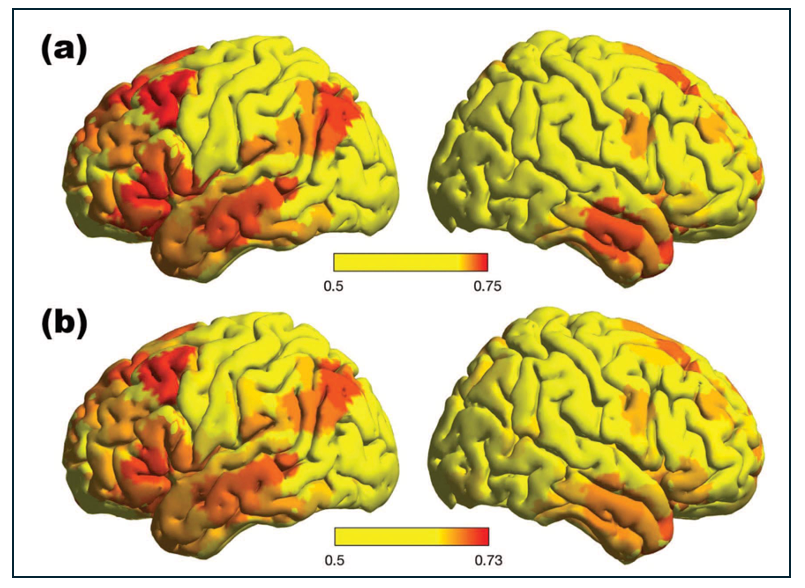
\includegraphics[width=\linewidth]{sex_classification.png}
  \caption{ROI-based sex classification shows high accuracies for (a) within sample CV and (b) across sample classification.}
  \label{fig:sexclass}
\end{wrapfigure}
and then infer which brain networks contribute most to distinguishing females from males.
\par\vspace{-1\parskip}\noindent
Our own ML work identified regionally specific networks with predictive power strongest in higher-level regions 
for language, social cognition, and emotion processing 
\parencite{weisSexClassificationResting2020a,wierschAccurateSexPrediction2023a,wierschSexDifferencesBrain2021a}.
However, RS primarily reflects intrinsic, trait-like brain organization. \\
What remains largely unexplored are 
sex differences in the “brain in action” when engaging with complex, multimodal input resembling real life. 
The present proposal aims to contribute to closing this gap in knowledge by applying the newly 
emerging NV approach to examine sex-specific brain responses in ecologically valid contexts. 
NV focuses on 
cognitive processes in dynamic, temporally extended, naturalistic contexts, which are much more akin to
situations which the brain must deal with in real life.
\par\vspace{-0.5\parskip}\noindent % small, controlled separation
Importantly, as opposed to RS, all participants are exposed to the same stimulus, 
for which content and timing 
is known and can be used in the analyses.
\par\vspace{-1\parskip}\noindent
NV approaches offer complex, dynamic and ongoing stimulation similar 
to experiences in everyday situations, where low-level (audiovisual) and high-level (cognitive and emotional) 
content vary fluidly, creating a multimodal and immersive experience 
\parencite{sonkusareNaturalisticStimuliNeuroscience2019}, offering the 
opportunity to capture dynamic neural processing in ecologically valid contexts 
\parencite{vanderwalMoviesMagnetNaturalistic2019} and has been shown to enhance reliability and 
identifiability compared to RS \parencite{krollNaturalisticViewingIncreases2023}.\\
Our lab has pioneered NV analyses. We developed the Topography-based Predictive Framework (TOPF) 
\parencite{liTopographybasedPredictiveFramework2023a}, which extracts individual-specific evoked 
topographies and links them to behavior using ML. 
Applied to NV data, TOPF achieved up to 80\% accuracy in 
sex classification, with predictive regions tied to emotion, language, and higher cognition. 
These promising results highlight the potential of NV to uncover novel sex differences.\\
Surprisingly, to our knowledge, no study has yet used NV to systematically examine sex differences. 
In a previous publication \parencite{eickhoffClinicalApplicationsMovie2020a}, we have compared the potential of 
movies for the study of 
individual brain differences to a cardiac stress-test, 
i.e. to potentially provide a standardized way to study the whole organ while it works to compare function 
across different levels of intensity and demands. 
We therefore expect NV to expose sex differences across a wide range of real-life-like situations—social interactions, 
face and emotion perception \parencite{sonkusareNaturalisticStimuliNeuroscience2019}, 
or complex narratives—that TB or RS approaches cannot capture. 
While isolated cognitive processes as examined in TB fMRI might not reveal 
significant sex differences, the complex interplay of these processes - as engaged during movie watching - could 
highlight more pronounced differences between women and men. 
Careful stimulus annotation will further allow us to identify the specific features and networks driving these differences.\\
Using advanced neuroimaging and analysis methods, we aim to detect subtle but meaningful sex-related differences 
in brain activity and FC, that can inform our understanding of 
broader cognitive and behavioral differences between females and males. 
First, we will study FC patterns that emerge over several minutes of movie watching. Then, we will zoom in to
identify specific events that trigger differences between women and men, and examine how these differences 
unfold in brain networks over time.\\
This multi-layered approach — combining aggregated and time-resolved FC, network dynamics, and brain activity — offers 
a richer view of sex differences in the brain function. 
Results from the proposed project can shed new light on why cognitive and behavioral patterns differ 
between women and men, and why certain neurological and psychiatric disorders present differently across the sexes. 
Such knowledge may improve diagnostic precision and personalized treatments, and support sex-specific 
strategies in healthcare and education.\\
We are uniquely positioned to realize this project, as our lab has already acquired the Ju-MOVIES dataset, 
a rich NV fMRI resource with over 130 participants. It combines extended movie stimuli, 
hormone measures, and detailed scene annotations, providing an unparalleled foundation for 
uncovering sex differences in the brain.\\
For clarity, throughout this proposal “sex” refers to self-reported biological sex. 
We acknowledge that “gender identity”, i.e. the 
subjective identification of an individual as female, male, or one of the other gender identities which might 
be also fluid, also plays a significant role, but this lies 
beyond the scope of the present project.

\subsection*{Data: The Ju-MOVIES dataset}
The proposed work builds on the Ju-MOVIES dataset, which has already been acquired and is 
uniquely suited for investigating sex differences with a NV approach. Its richness and design make it an ideal foundation for the present project. 
Over the course of the project, further data will be collected.
The paradigm comprises seven Hollywood movie excerpts (8 - 10 minutes each) selected to capture diverse social 
interactions, complex situations, and evolving emotions (“Dirty Dancing”, “Scream”, “Dead Poets Society”, “Forrest Gump”, “Dead Man Walking”, “Life is Beautiful”, 
“The Good, the Bad, the Ugly”), as well as 12 shorter clips and two RS scans of about 9 minutes. \\
Stimuli were chosen to be long enough for participants to grasp the context and empathize with characters, 
ensuring ecological validity.\\
So far, data from 135 healthy participants (68 males, 18 - 35 years) have been collected 
on a 3T Siemens Prisma scanner
with a 64-channel head coil, using a T2w multiband echo planar imaging sequence with the 
following parameters: repetition time (TR) = 980ms, echo time (TE) = 30ms, flip angle = 70°, field of view 
(FOV) = 207 x 207mm, voxel size=2.2 x 2.2 x 2.0mm3, number of slices: 64, multiband acceleration factor=4, 
phase encoding direction=AP,  FoV=207mm). A mirror fixed on the head coil allows participants to see a screen used 
to display the movies. In-ear headphones are used for ear protection and to deliver the movie sound. 
Additionally, a structural T1w image is acquired using an MP-RAGE sequence (TR=2000ms, TE=2.45ms, TI=900ms, 
flip angle=8°, FoV: 256mm) yielding 1mm3 voxels.
Alongside fMRI and structural imaging, saliva samples were collected and analyzed for levels of cortisol, estradiol, progesterone,
\begin{wrapfigure}{r}{0.27\textwidth} % r = rechts, l = links
  \vspace{-10pt} % optional: kleine Korrektur, damit es bündig startet
  \includegraphics[width=\linewidth]{emotions_DMW_edited.png}
  \caption{Exemplary emotion annotation for one of the movie stimuli..}
  \label{fig:dmw}
\end{wrapfigure}
 and testosterone to account for hormone-related variability. 
Oral contraceptive use was documented in women.
The movies are richly annotated: 
emotion ratings from 44 additional participants (23 males, age 20-30 years)
for the six basic emotions (happiness, fear, surprise, sadness, disgust and anger \parencite{ekmanConstantsCulturesFace1971a}), 
sampled at 10 Hz confirmed that the stimuli evoke a wide spectrum of affective states. 
Further annotations by two independent raters include scene content: faces, bodies, male / female presenting characters, ethnicity of characters, presence of children, 
adults, crowds, hands, buildings, vehicles, food, landscapes, animals, plants, movement, social interactions, 
place (inside or outside / urban vs. non-urban), time of day (day or night), weather, presence of music and 
camera movements, enabling fine-grained mapping of movie features to neural responses.
Altogether, Ju-MOVIES offers a rare combination of naturalistic stimulation, hormone measures, 
and detailed scene-level annotations, providing an exceptionally strong basis for the proposed project.


\subsection*{Work Program and Research Methods}
The overarching goal of the proposed project is to complement existing research on sex differences in the brain by 
employing a NVapproach. This method promises new insights into sex differences in brain responses to complex, 
dynamically evolving situations—much closer to the demands the brain faces in real life. Our results can go beyond 
findings from both TB and RS studies and provide perspectives that previous approaches could not achieve. 
Specifically, we will identify which types of complex situations depicted in the movie stimuli give rise to the 
most pronounced sex differences. In subsequent steps, we will disentangle which narrative events within the 
movies drive these differences and examine how female and male brains respond differentially to the evolving storyline. 
We expect that this innovative approach, combining analyses of temporally aggregated 
FC, event-related responses, network dynamics and brain activity will yield important new insights into 
the multi-faceted spectrum of sex differences in the brain in action.\\
\textbf{WP1}will extend existing RS findings by examining sustained FC during NV across time periods of several 
minutes. Using a temporally aggregated FC approach, as commonly applied to RS data, this work will identify 
sex differences in “action brain states” and their underlying networks.\\
\textbf{WP2} will build on this by employing a time-resolved FC approach to detect temporally specific events 
that drive sex differences in the experience of complex situations. Leveraging detailed annotations of the 
movie content, we will characterize which types of situations give rise to pronounced sex differences and 
reveal sex-specific cognitive strategies in processing them.\\
\textbf{WP3} will focus on brain activation patterns rather than FC. Here, we will extract typical female 
and male brain responses within each brain region to the dynamically evolving movie content. This analysis will 
complement WP1 and WP2 by providing a direct account of how women's and men's brains differentially respond 
to unfolding narrative events.

\subsection*{WP 1: The Brain in Action - The Naturalistic Viewing Action State (NV-AS)}

\textbf{Aim:} Identify sex differences in sustained, content-driven brain “action states” during NV 
and compare their predictive power against RS connectivity.

\textbf{Open Question:} Do sex-specific movie feature networks differ systematically, and if so, 
what do these differences reveal about distinct cognitive strategies in women and men?  

RS studies have shown that sex can be classified with high accuracy from temporally aggregated FC 
patterns \parencite{casanovaCombiningGraphMachine2012a,ritchieSexDifferencesAdult2018,weisSexClassificationResting2020a,wierschAccurateSexPrediction2023a,wierschSexDifferencesBrain2021a}. 
Because RS reflects brain activity in the absence of external stimulation, these patterns are often 
interpreted as proxies for intrinsic brain organization—capturing traits rather than actual states.\\ 
In this WP, we extend beyond RS by examining sustained FC patterns evoked by complex movie narratives. 
Unlike RS, these naturalistic viewing action states (NV-ASs) are content-driven: the brain's functional organization 
adapts to ongoing events in the film. Since the content is precisely known, we can link it to FC patterns and 
identify sex-specific differences in how these states unfold. 
Thus, this WP will provide insights into which kinds of complex situations elicit the strongest sex differences in 
brain networks. 
By focusing on the brain “in action,” we aim to capture sex differences in the overall experience of 
complex situations—an approach that is fundamentally different from both task-based studies 
(specific, isolated processes) and RS studies (intrinsic organization during free thought). 
We hypothesize that putting the brain into action will highlight sex differences more strongly than the 
unconstrained state of mind wandering \parencite{vanderwalIndividualDifferencesFunctional2017}.\\
Methodologically, we will adopt and extend our previous sex classification pipeline \parencite{weisSexClassificationResting2020a}. 
fMRI data will be parcellated \parencite{schaeferLocalGlobalParcellationHuman2018}, parcel-wise time courses extracted, 
and FC patterns computed. For each parcel, FC with the rest of the brain will serve as features for 
sex classification using cross-validation (CV), yielding a spatial map of classification accuracies for RS and 
each NV-AS (i.e., each movie).
Importantly, and in contrast to the majority of previous studies, we will incorporate hormone levels and oral contraceptive (OC) status in women as confounds in all 
prediction analyses to ensure that observed differences reflect sex per se rather than hormone-related variability. 
We will also implement rigorous strategies to prevent confound leakage \parencite{hamdanConfoundleakageConfoundRemoval2022a}, 
ensuring robust and unbiased results.

\subsubsection*{WP 1.1:  Comparing sex classification accuracies between RS and NV-ASs}
As a first step, we will compare sex classification performance between RS and NV-AS (averaged across all movies) 
within each parcel using corrected resampled \textit{t}-tests \parencite{nadeauInferenceGeneralizationError2003a}. 
Higher accuracies during NV relative to RS would indicate that sex differences emerge more strongly when the brain 
is “in action” rather than in its intrinsic resting organization.\\  
In addition, the spatial distribution of highly discriminative parcels in NV will highlight the brain 
networks underlying these sex differences. Their associated cognitive domains will be characterized using 
functional decoding \parencite{foxMetaanalysisHumanNeuroimaging2014a}.\\  
While sex differences in RS have often been reported in the default mode network (DMN) 
\parencite{weisSexClassificationResting2020a,zhangFunctionalConnectivityPredicts2018}, 
we expect NV-AS to reveal effects in higher cognitive or task-general networks 
\parencite{hugdahlExistenceGeneralizedNonspecific2015a}. 
Moreover, we hypothesize that sex classification based on NV-AS will outperform RS, 
consistent with findings for other phenotypes 
\parencite{finnCanBrainState2017a,vanderwalIndividualDifferencesFunctional2017} 
and with evidence that NV enhances individual identifiability over RS \parencite{krollNaturalisticViewingIncreases2023}.  

\subsubsection*{WP 1.2: Which movie features drive sex classification accuracies?}
To examine which kinds of complex situations maximize sex differences in the brain, we will characterize 
each movie clip by a set of visual and auditory features across its duration. 
These will include low-level properties such as mean motion energy, visual brightness, 
and auditory loudness, as well as higher-level properties such as number of faces, 
social interactions, and spoken words, which can be automatically extracted 
\parencite{mcnamaraDevelopingComprehensiveFramework2017a,radfordRobustSpeechRecognition2022}, 
alongside additional features from our manual annotations.\\  
We will then use a multiple regression approach to compare sex classification accuracies across the whole 
brain between the different movie clips. This analysis will delineate which movie features drive 
classification performance for each brain parcel. Because higher classification accuracy reflects more 
pronounced sex differences, this procedure will yield a “movie feature profile” that explains which 
features evoke the strongest differences.\\  
By clustering parcels according to their feature profiles, we will identify brain networks in which 
sex differences are jointly driven by specific features. We hypothesize that some of these networks will 
align with well-established cognitive domains (e.g., language, spatial cognition 
\parencite{halpernSexDifferencesCognitive2000a,kimuraSexCognition2000a}), whereas others will 
involve more generalized, task-independent resources \parencite{hugdahlExistenceGeneralizedNonspecific2015a}. 
We expect domain-specific networks to achieve higher classification accuracies than domain-general ones.\\ 
Finally, in an exploratory step, we will compare the expression of these networks in females and males. 
By computing the first principal component of each network’s FC pattern separately for women and men, 
we will derive “typical” female and male network signatures for each movie feature cluster. 
This analysis will reveal sex-specific cognitive strategies in response to complex, life-like situations.

\subsection*{WP 2: Going dynamic: Sex differences in time-resolved FC}

\textbf{Aim:} Determine which specific narrative events drive sex differences in FC 
and reveal sex-specific cognitive strategies in processing complex situations.  

\textbf{Open Questions:} How do naturalistic sex differences observed here relate to findings 
from traditional TB paradigms (e.g., isolated face viewing)? Do the same brain regions emerge, 
or do new networks appear under ecologically valid conditions?  

While WP1 examines sex differences in sustained “action states” evoked by movies, 
WP2 takes advantage of one of the main strengths of naturalistic viewing: its continuous, 
dynamic variation in content. Unlike RS or aggregated NV analyses, here the goal is to dissect 
the evolving brain responses to specific narrative events within the movies. 
Because all participants experience the same time-locked stimulus, the impact of movie content on the 
brain can be examined directly and with temporal precision. This enables us to move beyond asking whether 
men and women differ “on average” in their processing of complex situations, and 
instead pinpoint *which moments* in the evolving narrative trigger sex-specific brain network configurations. 
In other words, this WP shifts the focus from “what kind of situations” (WP1) to “exactly when and how” 
sex differences manifest during real-life-like experiences.\\  
Methodologically, fMRI data will again be parcellated, and parcel-wise time courses used to compute 
moment-by-moment co-fluctuations between regions using the edge time series (eTS) approach 
\parencite{betzelLivingEdgeNetwork2023a,faskowitzEdgecentricFunctionalNetwork2020a}. 
This effectively “unwraps” FC into its temporal evolution, yielding a time series of 
co-fluctuation magnitudes for each edge.\\
To identify dynamic FC differences between females and males during movie watching, we will identify
time points within the movies, at which females' and males' FC patterns are most distinct. To do so, we
will employ a ML approach at each time point to classify sex based on the individual time resolved FC
patterns. Given that the dimensionality of these features, i.e. the number of edges, is extremely high, we
will first employ a principal component analysis (PCA) for dimensionality reduction. Then, for each time
point, the first n (e.g. 50) principal components will be used as features to train a sex classifier for which
classification accuracy will be determined by use of a CV approach. Again, hormone levels and OC status
will be included in the models as confounds to control for hormone related variability and possible confound
leakage will be assessed and controlled for \parencite{hamdanConfoundleakageConfoundRemoval2022a}.\\
Significant time points—those at which classification exceeds chance level (p < 0.05 by permutation test)—will be 
taken as markers of narrative events that drive the strongest sex differences. 
To characterize these events, movie annotations will be used to code the presence of discrete features 
(e.g., faces, bodies, animals, scene cuts) and continuous features (e.g., luminance, audio intensity). 
Each significant time point will thus be linked to a detailed movie feature vector.  
We will then cluster significant time points across movies according to their feature vectors, 
thereby identifying categories of scenes that consistently evoke sex-specific differences. 
For each cluster, typical female and male FC patterns will be computed as the first principal component 
across participants, and thresholded to highlight the most discriminative connections and key network nodes. 
This will allow us to identify brain networks that respond differently in women and men to particular 
types of naturalistic events.\\
Altogether, WP2 will reveal which narrative elements most strongly drive sex differences in time-resolved 
FC and how these differences are expressed at the network level. 
While some of the observed patterns are expected to overlap with domains already known from TB studies 
(e.g., sex differences in face perception), this dynamic, ecologically valid approach will provide a 
much richer picture—capturing sex-specific strategies for processing complex, multimodal real-life situations.
Sex specific brain network patterns will potentially shed light on different cognitive strategies used by
females in males in dealing with complex real life-like events.   

\subsection*{WP 3: Shared but unique: Examination of the sex specific shared response to dynamic emotions}
\textbf{WP3 Aim: To characterize how female and male brains differ in their regional activation patterns to
evolving movie content, complementing connectivity-based analyses from WP1 and WP2.}\\
One of the main advantages of NV paradigms over the RS approach is that all participants are exposed to
the same stimulus, resulting in a synchronization of the neural response across participants. However, at
the same time, substantial individual differences within this 
response are preserved \parencite{finnIdiosynchronySharedResponses2020a,vanderwalIndividualDifferencesFunctional2017}. 
In this WP, instead of looking at time resolved FC patterns, we will focus directly
on the evolution of the neural response over time to examine in more detail, whether and how females' and
males' brains differ in response to the dynamic movie content. Considering that sex differences in emotion
perception and regulation have often been suggested in the literature 
(e.g. \parencite{domesNeuralCorrelatesSex2010a,gardenerSexDifferencesEmotion2013a})
and that movies are particularly effective in inducing strong negative and positive emotions
\parencite{grossEmotionElicitationUsing1995,westermannRelativeEffectivenessValidity1996}, we will 
focus on the sex differences in the brain's reaction
to the evolving emotional content over the course of the movies' narratives. Results from this WP will
extend existing findings on sex differences in emotion perception which have mostly only focused on single
emotions in rather artificial situations.\\
To do so, we will employ the new analysis approach (TOPF, \parencite{liTopographybasedPredictiveFramework2023a}) 
which has recently been developed in our lab. Simply speaking, for each brain region, this
methodological approach extracts the
shared brain response time course across a group of participants (through use of a PCA), which is evoked
by watching the movie. Furthermore, the individual expression of this shared response is computed, which
indicates to what extent the individual brain reaction matches the typical brain response across the group.
In the present context, we will employ an adjusted “two group” version of TOPF. Instead of identifying the
shared brain response across all participants, we will identify typical brain responses for females and males
separately. Importantly, to control for hormone related variance within the data, we will regress each
subject's time series on their hormone levels and use the residuals, i.e. the part of the signal not explained
by hormones, for computation of the shared response.
For each brain region we will compare the typical female and male response in two steps: Firstly, we will
check whether the typical female response is significantly different from the typical male response. This
will identify brain regions, in which the evoked brain response to movie differs fundamentally between
females and males. To further explore whether depicted emotions are the driving factor in differential brain
activation patterns in females and males we will employ the existing emotion annotation of our movies with
respect to the six basic emotions. For each of the brain regions which display significantly different time
courses for female and males, we will correlate the female and male time course with the emotion
annotation to find out which emotions drive the differences. High correlation between the female
respectively male shared response and annotation of specific emotions will identify emotions within the
movies that drive sex differences in certain parts of the brain.\\
For brain regions, where the overall sex specific brain responses do not differ significantly, we will compare
the individual expressions of this response by a two-sample t-test. This will identify brain regions, which
react to the narrative of the movie in a similar way, but in which the intensity of the experience differs
between females and males. We expect to find both types of regions mainly in higher cognitive regions,
which we will further explore through the use of functional decoding \parencite{foxMetaanalysisHumanNeuroimaging2014a}.
Finally, we aim to find out whether, across the whole brain, females and males differ fundamentally in their
perception of the evolving narrative of the movies. To this aim, for each subject, we will compute the
similarity of individual brain response to the sex-specific typical response for each brain region. Then we
will calculate a summary score (over all regions) to determine the sex of the subject by assigning them to
the class with the higher overall similarity score. If this classification works with high accuracy, it can be
taken to indicate, that there are typical female and male whole brain patterns in the perception of complex
narratives. Should this not be the case it would speak to the brain patterns being driven by individual factors
over sex.\\
\textbf{Main Goal: Identify sex-specific patterns in neural responses to dynamic emotional content during NV,
revealing how females and males process emotionally charged situations differentially.}\\
\textbf{Open Question 1 - Which Brain Regions Show Fundamental Sex Differences? Which brain regions
exhibit fundamentally different time-resolved responses to emotional content between females and males,
and are these differences consistent across movie narratives?}\\
\textbf{Open Question 2 - Which Emotions Drive Neural Divergence? Are specific emotional categories (e.g.,
fear, anger, happiness) more likely to induce divergent neural responses between females and males?}\\




\printbibliography

\end{document}
